\documentclass[10pt]{article}
\usepackage[polish]{babel}
\usepackage[utf8]{inputenc}
\usepackage[T1]{fontenc}
\usepackage{graphicx}
\usepackage[export]{adjustbox}
\graphicspath{ {./images/} }
\usepackage{amsmath}
\usepackage{amsfonts}
\usepackage{amssymb}
\usepackage[version=4]{mhchem}
\usepackage{stmaryrd}
\usepackage{multirow}

\title{EGZAMIN MATURALNY Z MATEMATYKI }

\author{}
\date{}


\begin{document}
\maketitle
Arkusz zawiera informacje prawnie chronione do momentu rozpoczęcia egzaminu.

KOD\\
PESEL\\
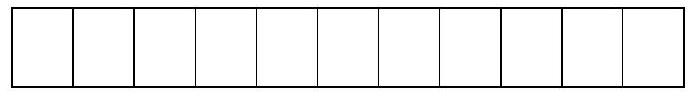
\includegraphics[max width=\textwidth, center]{2024_11_21_ebf83f11df6f4915f701g-01}\\
\(\square\)

\section*{POZIOM ROZSZERZONY}
\section*{Instrukcja dla zdającego}
\begin{enumerate}
  \item Sprawdź, czy arkusz egzaminacyjny zawiera 22 strony (zadania 1-12). Ewentualny brak zgłoś przewodniczącemu zespołu nadzorującego egzamin.
  \item Rozwiązania zadań i odpowiedzi wpisuj w miejscu na to przeznaczonym.
  \item Pamiętaj, że pominięcie argumentacji lub istotnych obliczeń w rozwiązaniu zadania otwartego może spowodować, że za to rozwiązanie nie otrzymasz pełnej liczby punktów.
  \item Pisz czytelnie i używaj tylko długopisu lub pióra z czarnym tuszem lub atramentem.
  \item Nie używaj korektora, a błędne zapisy wyraźnie przekreśl.
  \item Pamiętaj, że zapisy w brudnopisie nie będą oceniane.
  \item Możesz korzystać z zestawu wzorów matematycznych, cyrkla i linijki oraz kalkulatora prostego.
  \item Na tej stronie oraz na karcie odpowiedzi wpisz swój numer PESEL i przyklej naklejkę z kodem.
  \item Nie wpisuj żadnych znaków w części przeznaczonej dla egzaminatora.
\end{enumerate}

UZUPELNIA ZESPÓŁ NADZORUJĄCY\\
Uprawnienia zdającego do:\\

\includegraphics[max width=\textwidth, center]{2024_11_21_ebf83f11df6f4915f701g-01(1)}\\
dostosowania kryteriów oceniania\\
nieprzenoszenia zaznaczeń na kartę

7 MAJA 2020

Godzina rozpoczęcia:\\
9:00

Czas pracy:\\
180 minut

Liczba punktów do uzyskania: 50

MMA-R1\_1P-202

\section*{Zadanie 1. (4 pht)}
Rozwiąż nierówność \(\left(\frac{1}{x}-1\right)^{-1} \leq 1\).\\

\includegraphics[max width=\textwidth, center]{2024_11_21_ebf83f11df6f4915f701g-02}

Odpowiedź:

\section*{Zadanie 2. (3 pkt)}
Wyznacz wszystkie wartości parametru \(a\), dla których równanie \(|x-5|=(a-1)^{2}-4\) ma dwa różne rozwiązania dodatnie.\\

\includegraphics[max width=\textwidth, center]{2024_11_21_ebf83f11df6f4915f701g-03}

Odpowiedź: \(\qquad\)

\begin{center}
\begin{tabular}{|c|l|c|c|}
\hline
\multirow{2}{*}{\begin{tabular}{c}
Wypelnia \\
egzaminator \\
\end{tabular}} & Nr zadania & 1. & 2. \\
\cline { 2 - 4 }
 & Maks. liczba pkt & \(\mathbf{4}\) & \(\mathbf{3}\) \\
\cline { 2 - 4 }
 & Uzyskana liczba pkt &  &  \\
\hline
\end{tabular}
\end{center}

\section*{Zadanie 3. (3 pkt)}
Liczby dodatnie \(a\) i \(b\) spełniają równość \(a^{2}+2 a=4 b^{2}+4 b\). Wykaż, że \(a=2 b\).\\

\includegraphics[max width=\textwidth, center]{2024_11_21_ebf83f11df6f4915f701g-04}

\section*{Zadanie 4. (3 pht)}
Dany jest trójkąt równoramienny \(A B C\), w którym \(|A C|=|B C|=6\), a punkt \(D\) jest środkiem podstawy \(A B\). Okrąg o środku \(D\) jest styczny do prostej \(A C\) w punkcie \(M\). Punkt \(K\) leży na boku \(A C\), punkt \(L\) leży na boku \(B C\), odcinek \(K L\) jest styczny do rozważanego okręgu oraz \(|K C|=|L C|=2\) (zobacz rysunek).\\
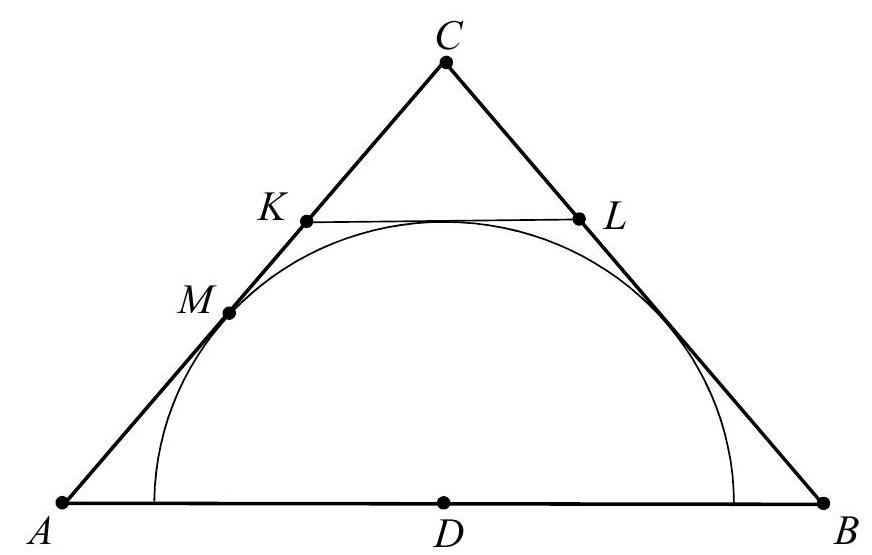
\includegraphics[max width=\textwidth, center]{2024_11_21_ebf83f11df6f4915f701g-05}

Wykaż, że \(\frac{|A M|}{|M C|}=\frac{4}{5}\).\\

\includegraphics[max width=\textwidth, center]{2024_11_21_ebf83f11df6f4915f701g-05(1)}

\begin{center}
\begin{tabular}{|l|l|c|c|}
\hline
\multirow{3}{*}{\begin{tabular}{l}
Wypetnia \\
egzaminator \\
\end{tabular}} & Nr zadania & 3. & 4. \\
\cline { 2 - 4 }
 & Maks. liczba pkt & 3 & 3 \\
\cline { 2 - 4 }
 & Uzyskana liczba pkt &  &  \\
\hline
\end{tabular}
\end{center}

\section*{Zadanie 5. (5 pht)}
W trzywyrazowym ciągu geometrycznym \(\left(a_{1}, a_{2}, a_{3}\right)\) spełniona jest równość \(a_{1}+a_{2}+a_{3}=\frac{21}{4}\).\\
Wyrazy \(a_{1}, a_{2}, a_{3}\) są - odpowiednio - czwartym, drugim i pierwszym wyrazem rosnącego ciągu arytmetycznego. Oblicz \(a_{1}\).\\

\includegraphics[max width=\textwidth, center]{2024_11_21_ebf83f11df6f4915f701g-06}\\

\includegraphics[max width=\textwidth, center]{2024_11_21_ebf83f11df6f4915f701g-07}

Odpowiedź: \(\qquad\)

\begin{center}
\begin{tabular}{|c|l|c|}
\hline
\multirow{2}{*}{\begin{tabular}{l}
Wypetnia \\
egzaminator \\
\end{tabular}} & Nr zadania & 5. \\
\cline { 2 - 3 }
 & Maks. liczba pkt & 5 \\
\cline { 2 - 3 }
 & Uzyskana liczba pkt &  \\
\hline
\end{tabular}
\end{center}

\section*{Zadanie 6. (4 pkt)}
Rozwiąż równanie \(3 \cos 2 x+10 \cos ^{2} x=24 \sin x-3\) dla \(x \in\langle 0,2 \pi\rangle\).\\

\includegraphics[max width=\textwidth, center]{2024_11_21_ebf83f11df6f4915f701g-08}\\

\includegraphics[max width=\textwidth, center]{2024_11_21_ebf83f11df6f4915f701g-09}

Odpowiedź: \(\qquad\)

\begin{center}
\begin{tabular}{|c|l|c|}
\hline
\multirow{2}{*}{\begin{tabular}{c}
Wypetnia \\
egzaminator \\
\end{tabular}} & Nr zadania & \(\mathbf{6 .}\) \\
\cline { 2 - 3 }
 & Maks. liczba pkt & 4 \\
\cline { 2 - 3 }
 & Uzyskana liczba pkt &  \\
\hline
\end{tabular}
\end{center}

\section*{Zadanie 7. (4 pkt)}
Dane jest równanie kwadratowe \(x^{2}-(3 m+2) x+2 m^{2}+7 m-15=0\) z niewiadomą \(x\). Wyznacz wszystkie wartości parametru \(m\), dla których różne rozwiązania \(x_{1}\) i \(x_{2}\) tego równania istnieją i spełniają warunek

\[
2 x_{1}^{2}+5 x_{1} x_{2}+2 x_{2}^{2}=2 .
\]


\includegraphics[max width=\textwidth, center]{2024_11_21_ebf83f11df6f4915f701g-10}\\

\includegraphics[max width=\textwidth, center]{2024_11_21_ebf83f11df6f4915f701g-11}

Odpowiedź:

\begin{center}
\begin{tabular}{|c|l|c|}
\hline
\multirow{2}{*}{\begin{tabular}{l}
Wypelnia \\
egzaminator \\
\end{tabular}} & Nr zadania & 7. \\
\cline { 2 - 3 }
 & Maks. liczba pkt & 4 \\
\cline { 2 - 3 }
 & Uzyskana liczba pkt &  \\
\hline
\end{tabular}
\end{center}

\section*{Zadanie 8. (4 pht)}
W trójkącie równoramiennym \(A B C:|A C|=|B C|=10\), a miara kąta \(A B C\) jest równa \(30^{\circ}\).\\
Na boku \(B C\) wybrano punkt \(P\), taki, że \(\frac{|B P|}{|P C|}=\frac{2}{3}\). Oblicz sinus kąta \(\alpha\) (zobacz rysunek).\\
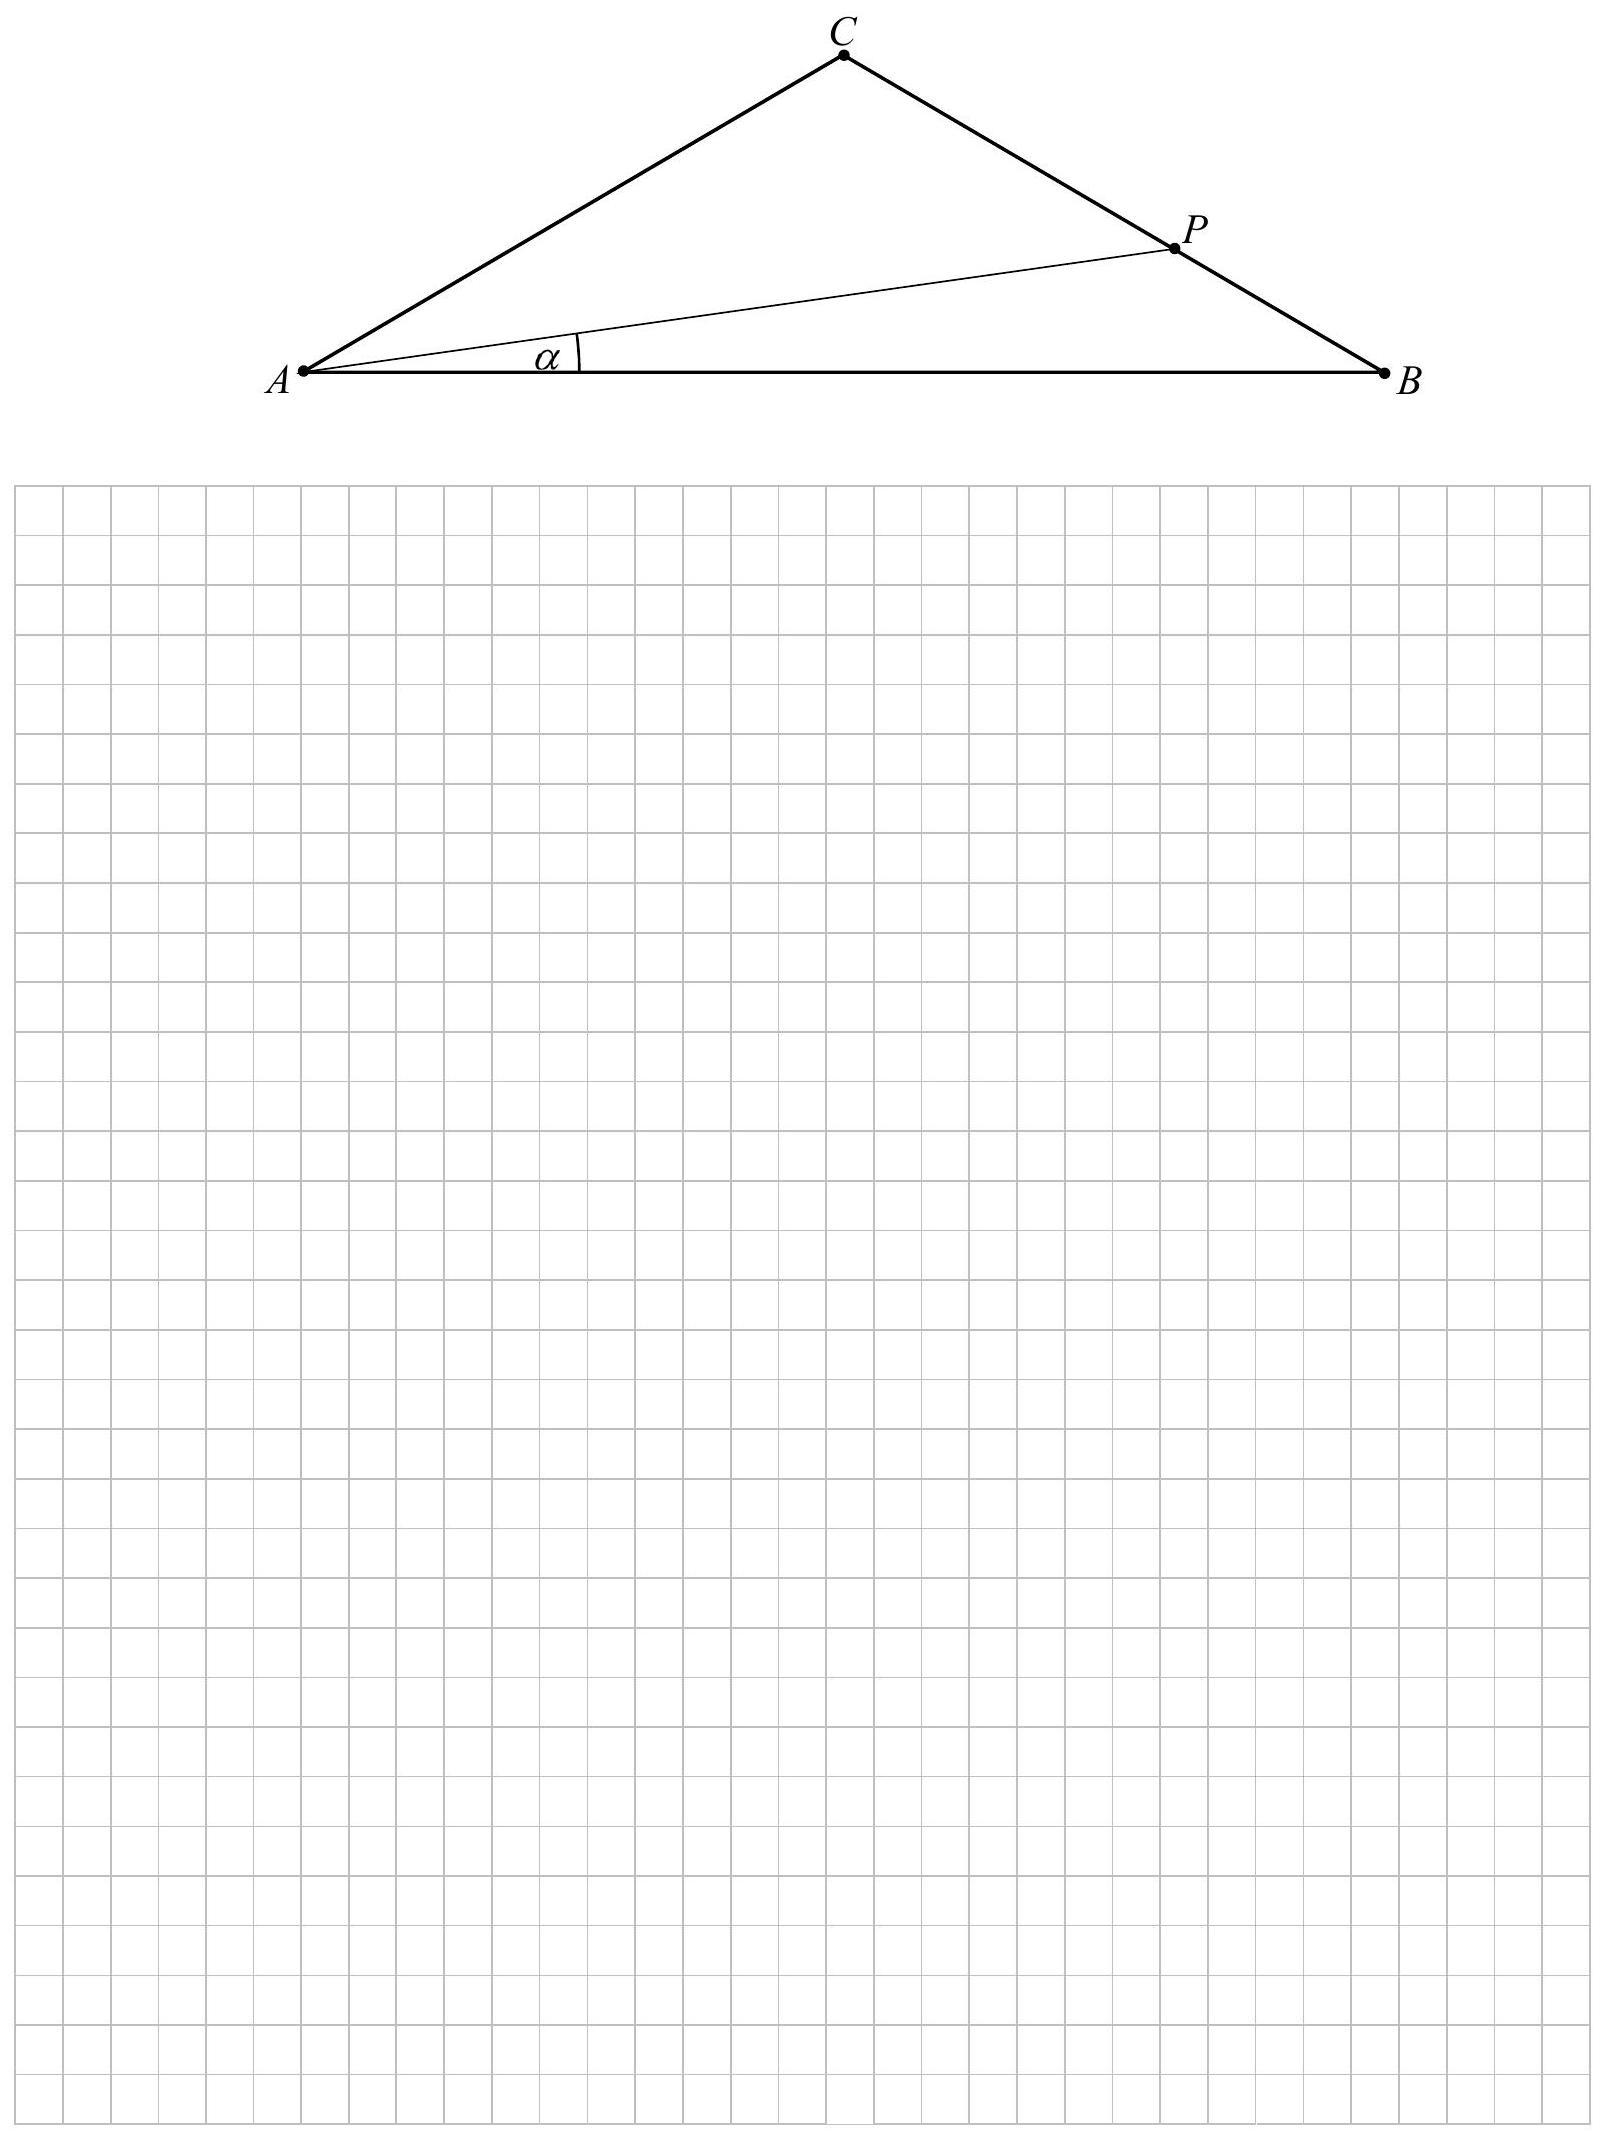
\includegraphics[max width=\textwidth, center]{2024_11_21_ebf83f11df6f4915f701g-12}\\

\includegraphics[max width=\textwidth, center]{2024_11_21_ebf83f11df6f4915f701g-13}

Odpowiedź: \(\qquad\)

\begin{center}
\begin{tabular}{|c|l|c|}
\hline
\multirow{2}{*}{\begin{tabular}{l}
Wypetnia \\
egzaminator \\
\end{tabular}} & Nr zadania & \(\mathbf{8 .}\) \\
\cline { 2 - 3 }
 & Maks. liczba pkt & \(\mathbf{4}\) \\
\cline { 2 - 3 }
 & Uzyskana liczba pkt &  \\
\hline
\end{tabular}
\end{center}

\section*{Zadanie 9. (5 pkt)}
Prosta o równaniu \(x+y-10=0\) przecina okrąg o równaniu \(x^{2}+y^{2}-8 x-6 y+8=0\) w punktach \(K\) i \(L\). Punkt \(S\) jest środkiem cięciwy \(K L\). Wyznacz równanie obrazu tego okręgu w jednokładności o środku \(S\) i skali \(k=-3\).\\

\includegraphics[max width=\textwidth, center]{2024_11_21_ebf83f11df6f4915f701g-14}\\

\includegraphics[max width=\textwidth, center]{2024_11_21_ebf83f11df6f4915f701g-15}

Odpowiedź:

\begin{center}
\begin{tabular}{|c|l|c|}
\hline
\multirow{2}{*}{\begin{tabular}{l}
Wypelnia \\
egzaminator \\
\end{tabular}} & Nr zadania & 9. \\
\cline { 2 - 3 }
 & Maks. liczba pkt & 5 \\
\cline { 2 - 3 }
 & Uzyskana liczba pkt &  \\
\hline
\end{tabular}
\end{center}

\section*{Zadanie 10. (5 pkt)}
Dany jest kwadrat \(A B C D\) o boku długości 2. Na bokach \(B C\) i \(C D\) tego kwadratu wybrano - odpowiednio - punkty \(P\) i \(Q\), takie, że długość odcinka \(|P C|=|Q D|=x\) (zobacz rysunek). Wyznacz tę wartość \(x\), dla której pole trójkąta \(A P Q\) osiąga wartość najmniejszą. Oblicz to najmniejsze pole.\\
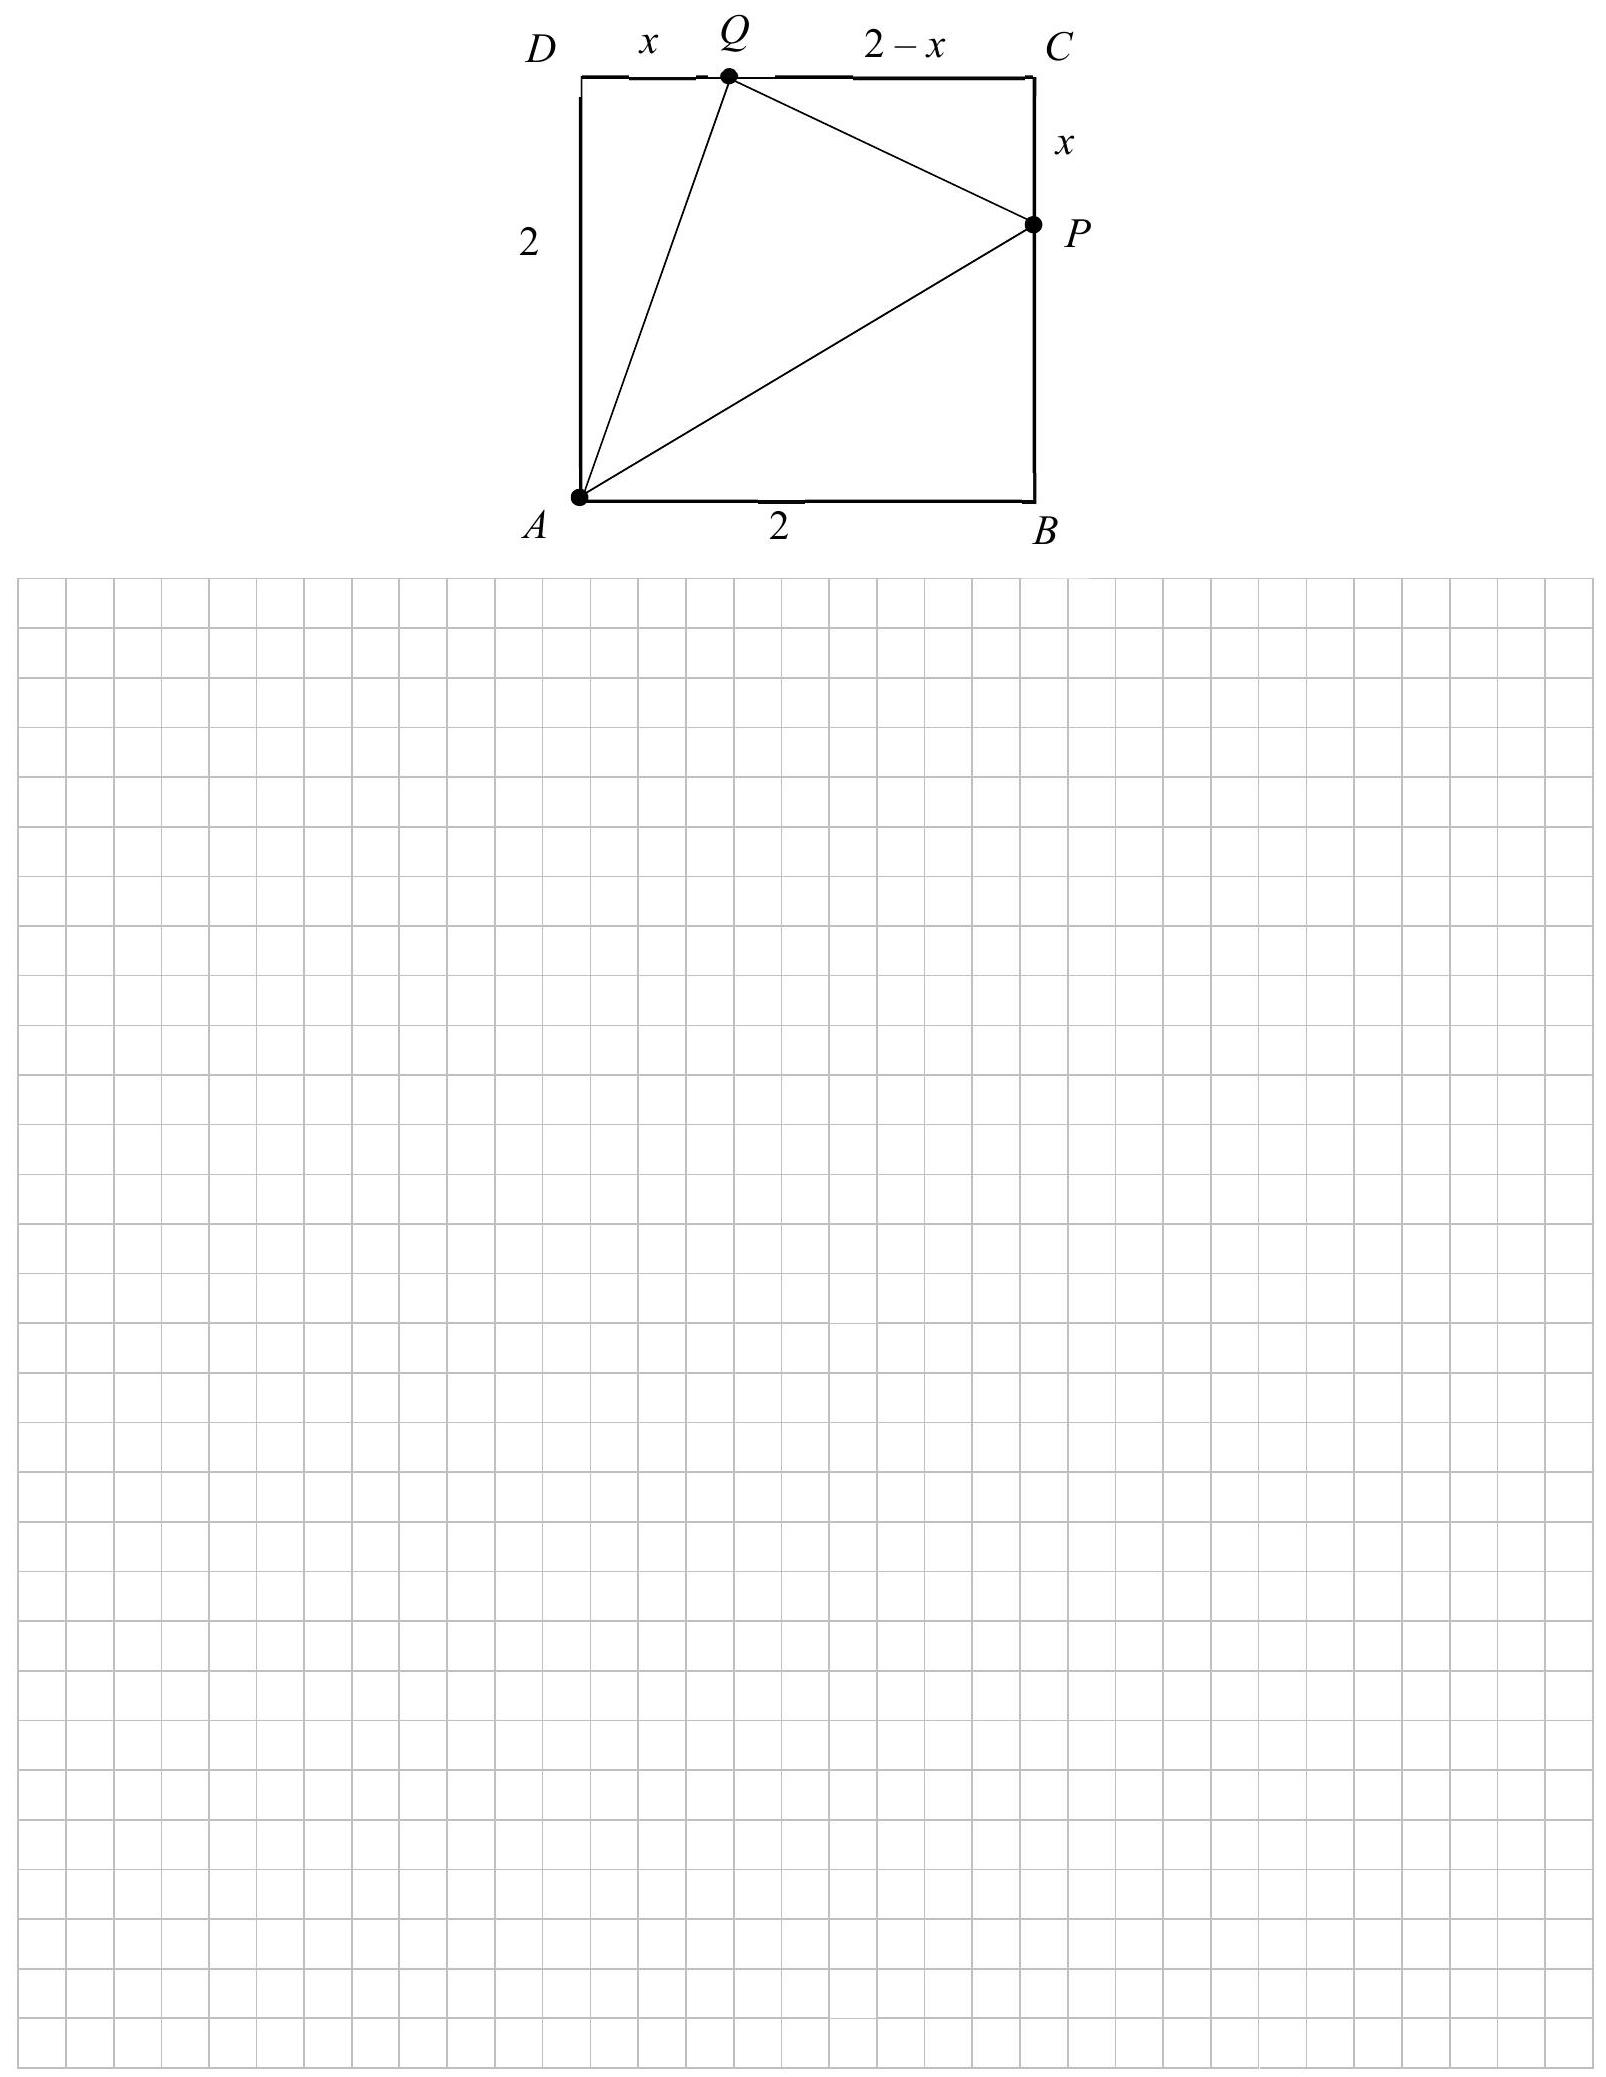
\includegraphics[max width=\textwidth, center]{2024_11_21_ebf83f11df6f4915f701g-16}\\

\includegraphics[max width=\textwidth, center]{2024_11_21_ebf83f11df6f4915f701g-17}

Odpowiedź: \(\qquad\)

\begin{center}
\begin{tabular}{|c|l|c|}
\hline
\multirow{2}{*}{\begin{tabular}{l}
Wypelnia \\
egzaminator \\
\end{tabular}} & Nr zadania & 10. \\
\cline { 2 - 3 }
 & Maks. liczba pkt & 5 \\
\cline { 2 - 3 }
 & Uzyskana liczba pkt &  \\
\hline
\end{tabular}
\end{center}

\section*{Zadanie 11. (4 pkt)}
Oblicz, ile jest wszystkich siedmiocyfrowych liczb naturalnych, w których zapisie dziesiętnym występują dokładnie trzy cyfry 1 i dokładnie dwie cyfry 2.\\

\includegraphics[max width=\textwidth, center]{2024_11_21_ebf83f11df6f4915f701g-18}\\

\includegraphics[max width=\textwidth, center]{2024_11_21_ebf83f11df6f4915f701g-19}

Odpowiedź:

\begin{center}
\begin{tabular}{|c|l|c|}
\hline
\multirow{2}{*}{\begin{tabular}{l}
Wypelnia \\
egzaminator \\
\end{tabular}} & Nr zadania & 11. \\
\cline { 2 - 3 }
 & Maks. liczba pkt & 4 \\
\cline { 2 - 3 }
 & Uzyskana liczba pkt &  \\
\hline
\end{tabular}
\end{center}

\section*{Zadanie 12. (6 pkt)}
Podstawą ostrosłupa czworokątnego \(A B C D S\) jest trapez \(A B C D(A B \| C D)\). Ramiona tego trapezu mają długości \(|A D|=10\) i \(|B C|=16\), a miara kąta \(A B C\) jest równa \(30^{\circ}\). Każda ściana boczna tego ostrosłupa tworzy z płaszczyzną podstawy kąt \(\alpha\), taki, że \(\operatorname{tg} \alpha=\frac{9}{2}\). Oblicz objętość tego ostrosłupa.

\begin{center}
\begin{tabular}{|c|c|c|c|c|c|c|c|c|c|c|c|c|c|c|c|c|c|c|c|c|c|c|c|}
\hline
 &  &  &  &  &  &  &  &  &  &  &  &  &  &  &  &  &  &  &  &  &  &  &  \\
\hline
 &  &  &  &  &  &  &  &  &  &  &  &  &  &  &  &  &  &  &  &  &  &  &  \\
\hline
 &  &  &  &  &  &  &  &  &  &  &  &  &  &  &  &  &  &  &  &  &  &  &  \\
\hline
 &  &  &  &  &  &  &  &  &  &  &  &  &  &  &  &  &  &  &  &  &  &  &  \\
\hline
 &  &  &  &  &  &  &  &  &  &  &  &  &  &  &  &  &  &  &  &  &  &  &  \\
\hline
 &  &  &  &  &  &  &  &  &  &  &  &  &  &  &  &  &  &  &  &  &  &  &  \\
\hline
 &  &  &  &  &  &  &  &  &  &  &  &  &  &  &  &  &  &  &  &  &  &  &  \\
\hline
 &  &  &  &  &  &  &  &  &  &  &  &  &  &  &  &  &  &  &  &  &  &  &  \\
\hline
 &  &  &  &  &  &  &  &  &  &  &  &  &  &  &  &  &  &  &  &  &  &  &  \\
\hline
 &  &  &  &  &  &  &  &  &  &  &  &  &  &  &  &  &  &  &  &  &  &  &  \\
\hline
 &  &  &  &  &  &  &  &  &  &  &  &  &  &  &  &  &  &  &  &  &  &  &  \\
\hline
 &  &  &  &  &  &  &  &  &  &  &  &  &  &  &  &  &  &  &  &  &  &  &  \\
\hline
 &  &  &  &  &  &  &  &  &  &  &  &  &  &  &  &  &  &  &  &  &  &  &  \\
\hline
 &  &  &  &  &  &  &  &  &  &  &  &  &  &  &  &  &  &  &  &  &  &  &  \\
\hline
 &  &  &  &  &  &  &  &  &  &  &  &  &  &  &  &  &  &  &  &  &  &  &  \\
\hline
 &  &  &  &  &  &  &  &  &  &  &  &  &  &  &  &  &  &  &  &  &  &  &  \\
\hline
 &  &  &  &  &  &  &  &  &  &  &  &  &  &  &  &  &  &  &  &  &  &  &  \\
\hline
 &  &  &  &  &  &  &  &  &  &  &  &  &  &  &  &  &  &  &  &  &  &  &  \\
\hline
 &  &  &  &  &  &  &  &  &  &  &  &  &  &  &  &  &  &  &  &  &  &  &  \\
\hline
 &  &  &  &  &  &  &  &  &  &  &  &  &  &  &  &  &  &  &  &  &  &  &  \\
\hline
 &  &  &  &  &  &  &  &  &  &  &  &  &  &  &  &  &  &  &  &  &  &  &  \\
\hline
 &  &  &  &  &  &  &  &  &  &  &  &  &  &  &  &  &  &  &  &  &  &  &  \\
\hline
 &  &  &  &  &  &  &  &  &  &  &  &  &  &  &  &  &  &  &  &  &  &  &  \\
\hline
 &  &  &  &  &  &  &  &  &  &  &  &  &  &  &  &  &  &  &  &  &  &  &  \\
\hline
 &  &  &  &  &  &  &  &  &  &  &  &  &  &  &  &  &  &  &  &  &  &  &  \\
\hline
 &  &  &  &  &  &  &  &  &  &  &  &  &  &  &  &  &  &  &  &  &  &  &  \\
\hline
 &  &  &  &  &  &  &  &  &  &  &  &  &  &  &  &  &  &  &  &  &  &  &  \\
\hline
 &  &  &  &  &  &  &  &  &  &  &  &  &  &  &  &  &  &  &  &  &  &  &  \\
\hline
 &  &  &  &  &  &  &  &  &  &  &  &  &  &  &  &  &  &  &  &  &  &  &  \\
\hline
 &  &  &  &  &  &  &  &  &  &  &  &  &  &  &  &  &  &  &  &  &  &  &  \\
\hline
 &  &  &  &  &  &  &  &  &  &  &  &  &  &  &  &  &  &  &  &  &  &  &  \\
\hline
 &  &  &  &  &  &  &  &  &  &  &  &  &  &  &  &  &  &  &  &  &  &  &  \\
\hline
 &  &  &  &  &  &  &  &  &  &  &  &  &  &  &  &  &  &  &  &  &  &  &  \\
\hline
 &  &  &  &  &  &  &  &  &  &  &  &  &  &  &  &  &  &  &  &  &  &  &  \\
\hline
 &  &  &  &  &  &  &  &  &  &  &  &  &  &  &  &  &  &  &  &  &  &  &  \\
\hline
 &  &  &  &  &  &  &  &  &  &  &  &  &  &  &  &  &  &  &  &  &  &  &  \\
\hline
 &  &  &  &  &  &  &  &  &  &  &  &  &  &  &  &  &  &  &  &  &  &  &  \\
\hline
 &  &  &  &  &  &  &  &  &  &  &  &  &  &  &  &  &  &  &  &  &  &  &  \\
\hline
 &  &  &  &  &  &  &  &  &  &  &  &  &  &  &  &  &  &  &  &  &  &  &  \\
\hline
 &  &  &  &  &  &  &  &  &  &  &  &  &  &  &  &  &  &  &  &  &  &  &  \\
\hline
\end{tabular}
\end{center}

\begin{center}

\includegraphics[max width=\textwidth]{2024_11_21_ebf83f11df6f4915f701g-21}
\end{center}

Odpowiedź:

\begin{center}
\begin{tabular}{|c|l|c|}
\hline
\multirow{2}{*}{\begin{tabular}{l}
Wypelnia \\
egzaminator \\
\end{tabular}} & Nr zadania & 12. \\
\cline { 2 - 3 }
 & Maks. liczba pkt & 6 \\
\cline { 2 - 3 }
 & Uzyskana liczba pkt &  \\
\hline
\end{tabular}
\end{center}

\section*{BRUDNOPIS (nie podlega ocenie)}

\end{document}